\documentclass[reprint,amsmath,amssymb,aps,prd,nofootinbib,floatfix]{revtex4-2}

\usepackage{graphicx}
\usepackage{bm}
\usepackage{physics}
\usepackage{placeins}
\usepackage[nopatch=footnote]{microtype}

% Reduce minor underfull/overfull boxes without manual line-breaking
\setlength{\emergencystretch}{2em}

\begin{document}

\title{Minimal Point-Process Dynamics with Memory: Emergent Time and Metastable Structures}

\author{H. Horn}
\affiliation{Peine Stederdorf, Germany}

\date{28 February 2026} % explicit date for submissions/arXiv

\begin{abstract}
We propose a minimal stochastic dynamics on an abstract continuous state space $\Omega$ in which a trajectory $x_n$ is coupled to an explicit, finite, relaxing memory density $\rho_n$.
The memory update is generically non-invertible, yielding an intrinsic arrow of \emph{update order}.
Coarse-graining over $n\gg\alpha^{-1}$ motivates an effective parameter $t=\alpha n$ and, when a separation of scales is present, an approximate continuum SDE/Fokker--Planck description.
In this regime we introduce trajectory-based, coordinate-robust diagnostics (persistence/relaxation rates, dimensionless stability measures, and metastable residence-time statistics) to identify and compare long-lived localized dynamical structures induced by the endogenous memory coupling.
Calibration to spacetime units and connections to relativistic dynamics and Standard-Model-like structures are deferred to companion work.
\end{abstract}

\maketitle

%-------------------------------------------------
\section{Introduction}
%-------------------------------------------------

Modern fundamental physics rests on a small number of highly successful theoretical frameworks, in particular quantum field theory and general relativity.
Despite their empirical success, both rely on foundational structures---spacetime, quantum states, and fields---that are postulated rather than derived.

This becomes particularly apparent in attempts to unify quantum theory and gravitation.
A range of non-perturbative programs (e.g., asymptotic safety \cite{Weinberg1979,Reuter1998,NiedermaierReuter2006,Percacci2017}, causal sets \cite{Bombelli1987,Sorkin2003}, loop-based formulations \cite{Rovelli2004,AshtekarLewandowski2004}, and string theory \cite{Polchinski1998}) achieves internal consistency but typically assumes notions such as time, locality, or dimensionality from the outset \cite{Anderson1972,Laughlin2000}.

The present work is motivated by the hypothesis that these difficulties are not primarily technical, but conceptual.
Rather than postulating spacetime, quantum structure, or particles, we ask how such notions could arise from a more primitive irreversible dynamics.
Concretely, we assume only a sequence of non-trivial update events defining a trajectory in an abstract state space.

Related ideas appear in digital-physics approaches \cite{Wolfram2002,tHooft2016} and in history-dependent random-walk models \cite{Nelson1966,Pemantle2007,BenAImRaimond2002}.
Closest in spirit are self-interacting walks biased by their visitation history, such as the true (myopic) self-avoiding walk (TSAW) \cite{AmitParisiPeliti1983,TothWerner1998} and the self-repelling Brownian polymer (SRBP) \cite{DurrettRogers1992}; see also \cite{PelitiPietronero1987}.

While our model shares with these approaches the idea of a trajectory coupled to a self-generated field, it differs structurally: the memory is an explicit, finite, relaxing distribution updated by Eq.~(\ref{eq:memorydistribution}). This makes the update map generically non-invertible (information-losing) and thereby induces an intrinsic arrow of \emph{update order} at the fundamental level; that is, the full past cannot be reconstructed from the present state. (We intentionally distinguish this update-order arrow from any thermodynamic or relativistic notion of physical time, which is not assumed here.)
Memory and trajectory thus emerge jointly as the minimal departure from trivial dynamics, rather than being encoded in external boundary conditions.

By contrast, TSAW/SRBP-type formulations are typically written directly in terms of the full occupation history (or local time) without explicit forgetting \cite{AmitParisiPeliti1983,TothWerner1998,DurrettRogers1992,PelitiPietronero1987}.

\paragraph{Roadmap (conceptual to operational).}
We first give a brief motivation (without a formal proof) for why a locally linear, metric-like coarse-grained description is a natural attractor once one assumes only directed, comparable update steps (Sec.~\ref{sec:minimalist_motivation}); readers primarily interested in the model and diagnostics may skip directly to Sec.~\ref{sec:MinDynModel}.
In Sec.~\ref{sec:MinDynModel} we specify the minimal generator---a stochastic point process on $\Omega$ coupled to a finite, relaxing memory distribution.
Sec.~\ref{sec:EmergenceTime} introduces an effective coarse-grained time parametrization and discusses when a continuum description is useful.
Subsequent sections develop operational diagnostics (metastability, persistence/relaxation rates, and dimensionless stability measures) and analyze memory-induced irreversibility and the formation of robust, typically metastable dynamical structures.

A minimal reference implementation accompanies this work in the repository, with a NumPy-based finite-memory simulator, diagnostic functions, tests under `tests/`, and the reproducible runner `experiments/current/reference/reference_experiment.py` that support the reproducibility of the key numerical claims.

%-------------------------------------------------
\subsection{Minimalist motivation: from directed updates to effective geometry}\label{sec:minimalist_motivation}
%-------------------------------------------------

Our starting point is deliberately weak: we assume only (i) distinguishable events and (ii) a directed update order between them.
To compare elementary updates, we further assume that minimal transitions can be assigned increments $\Delta$ in some comparison set $\mathcal{S}$ and that concatenation of transitions induces an associative composition law.

The purpose of this subsection is to justify why it is reasonable to work with continuum notions later on.
Under mild regularity and coarse-graining assumptions---continuity, refinement invariance, and a central-limit-type scaling of fluctuations---a consistent composition law generically linearizes locally and yields a tangent-space-like description.
If fluctuations are approximately isotropic at the coarse-grained scale, the covariance further induces an effective inner product.
In short: differentiability and metric structure are treated as \emph{effective} notions arising from stable large-scale behavior, not as fundamental axioms.

In Paper~I we therefore work directly with a concrete minimal dynamics on a continuous state space $\Omega$.
The emergent coarse-grained geometry serves only as a consistency target and an interpretive guide for diagnostics extracted from trajectories.

% Bridge sentence absorbed into the roadmap above.
%\paragraph{Paper organization.}
%The paper follows the roadmap above.

%-------------------------------------------------
\section{Minimal Dynamical Model}\label{sec:MinDynModel}
%-------------------------------------------------

In this section we define the minimal dynamical framework underlying the present work.
No assumptions about spacetime, physical geometry, quantum mechanics, fields, or conserved quantities are made at this stage.

\subsection{Background structure and invariances}\label{sec:background_invariances}

The model is formulated on a continuous state space $\Omega$ equipped with a reference measure $dx$ and a choice of local coordinates sufficient to define integrals and derivatives.
In practice one may take $\Omega\subseteq\mathbb{R}^d$ with the Lebesgue measure and the Euclidean inner product.
This background structure is a minimal mathematical scaffold for writing the generator and the diagnostics; it is not assumed to be a fundamental physical spacetime metric.

Two distinct notions of ``invariance'' are relevant.
First, once the extended state is defined in Eq.~(\ref{eq:augmented_state}), the resulting process is Markov by construction, and the update order $n\mapsto n+1$ is physically meaningful because the memory update is generally non-invertible.
Second, many of the observables we use are designed to be operational and robust under benign reparametrizations of $\Omega$ (e.g., translations, rotations, and global rescalings in the chosen coordinate chart), in the sense that they depend on coarse-grained residence statistics and relaxation rates rather than on absolute coordinate values.

Quantities that explicitly use $\nabla$ (e.g., drifts of the form $-\nabla\Phi[\rho]$ and Hessian-based OU linearizations) depend on the chosen coordinate/inner-product structure and should be interpreted as part of the effective description.
Accordingly, whenever we invoke ``isotropy'' or compare rates across runs, we do so at the level of dimensionless ratios or fit parameters extracted from trajectory data, not by assuming a preferred physical metric on $\Omega$.

\subsection{Dynamical setup}

We consider a single generative process producing a sequence of states indexed by an integer update parameter $n\in\mathbb{N}$.
The parameter $n$ labels successive update steps of the process and does not represent physical time.

\subsection{State definition}

The full process state at update step $n$ is
\begin{equation} \label{eq:augmented_state}
z_n := (x_n,\rho_n).
\end{equation}

Here $x_n$ denotes the current position of the process, while $\rho_n$ represents a memory distribution encoding the influence of past states.

\paragraph{Notation (update index vs.\ time).}
We use $n\in\mathbb{N}$ for the discrete update index and reserve the word ``time'' for the coarse-grained parameter introduced later (Sec.~\ref{sec:EmergenceTime}). In Eq.~(\ref{eq:augmented_state}), $x_n\in\Omega$ is the current process position and $\rho_n$ is a normalized, non-negative \emph{memory density} on $\Omega$ (with respect to the reference measure $dx$). While $\rho_n$ is normalized like a probability density, in Paper~I it is primarily a bookkeeping device for finite, relaxing memory; its normalization fixes an overall scale and should not be read as an epistemic probability unless explicitly stated.

Assumptions on $\Omega$ (continuity, reference measure, and coordinate/inner-product scaffold) were fixed in Sec.~\ref{sec:background_invariances} and are used here as an effective parametrization for writing Eqs.~(\ref{eq:trajectory})--(\ref{eq:memorypotential}). Throughout Paper~I, $\Omega$ remains an abstract state space; any identification with physical space or spacetime geometry is deferred to companion work.

\subsection{Why a point process? (minimal carrier choice)}

The fundamental dynamical variable $x_n$ is chosen to be a single point in state space.
This is not meant as a physical claim that fundamental entities are point particles.
Rather, it is a minimal \emph{carrier} of sequential updates: any iterative generator must, at each step, select ``what happened'' in some configuration space, and a point-valued state is the simplest such representation.

Importantly, the formalism is not tied to this choice.
One may replace $x_n$ by (for example) a field configuration, a graph, a tuple of points, or a probability distribution; the same structural idea then becomes an irreversible update of a finite-memory variable coupled back into the generator.
We therefore view ``point'' as a design choice that makes the mechanism maximally transparent, not as an asserted inevitability.

The memory variable $\rho_n(x)$ is a normalized, non-negative density (with respect to a chosen reference measure $dx$),
\begin{equation}
\rho_n(x) \ge 0,
\qquad
\int_\Omega \rho_n(x)\,dx = 1,
\end{equation}
which we assume to be effectively localized (e.g., rapidly decaying outside a characteristic region). Implicitly, this normalization presumes either $\Omega=\mathbb{R}^d$ with sufficiently fast decay, or boundary conditions (e.g., periodic or reflecting) under which the update in Eq.~(\ref{eq:memorydistribution}) preserves total mass.

\subsection{Trajectory update rule}

The evolution of the position variable is governed by
\begin{equation}\label{eq:trajectory}
x_{n+1} = x_n + \varepsilon\,\xi_n - \eta\,\nabla\Phi_n(x_n).
\end{equation}

The appearance of $\nabla$ should be read as an effective smooth structure tied to the chosen coordinate chart on $\Omega$.
At the discrete level, one could equivalently replace the gradient by a local finite-difference/score-type rule on the coarse-graining scale $\sigma$; the use of $\nabla$ is a compact notation anticipating that the memory potential $\Phi_n$ is smooth once $\rho_n$ is a mixture of smooth kernels $G_\sigma$.
Thus, differentiability is not a fundamental assumption about ``spacetime,'' but a property of the coarse-grained interaction term induced by the memory update.

The stochastic variable $\xi_n$ is assumed to be isotropic and dimensionless, with unit variance \cite{Gardiner2009}. As in Sec.~\ref{sec:background_invariances}, ``isotropic'' is understood relative to the chosen coordinate/inner-product scaffold on $\Omega$, not as a fundamental physical postulate. The parameters $\varepsilon$ and $\eta$ control the relative strength of stochastic fluctuations and memory-induced drift.

\subsection{Memory update rule}
The memory distribution evolves according to
\begin{equation}\label{eq:memorydistribution}
\rho_{n+1}(x) = (1-\alpha)\rho_n(x) + \alpha\,G_\sigma(x-x_{n+1}),
\end{equation}
where $G_\sigma$ is a smooth, normalized kernel with finite width $\sigma$. The update rule is explicitly non-invertible.

\paragraph{Standing notation.}
Unless stated otherwise: $n\in\mathbb{N}$ denotes the discrete update index; $x_n\in\Omega$ the point-valued state; $\rho_n$ a probability density on $\Omega$ with respect to $dx$; $G_\sigma$ a normalized smoothing kernel (width $\sigma$); and $K$ an interaction kernel used to define the memory potential in Eq.~(\ref{eq:memorypotential}). We reserve the term ``time'' for the coarse-grained parameter introduced later (Sec.~\ref{sec:EmergenceTime}).

\begin{figure}[tbp]
    \centering
    
\includegraphics[width=0.72\linewidth]{../figures/paper/fig1_knot_trajectory.pdf}
    \caption{
    Memory-driven self-avoiding trajectory in a two-dimensional state space.
    The continuous line represents the full trajectory generated by the discrete update rules defined in Sec.~\ref{sec:MinDynModel}.
    Despite stochastic forcing, self-intersections are suppressed due to the accumulated memory.
    }
    \label{fig:2d_trajectory}
\end{figure}

For definiteness, one may assume that $G_\sigma$ is radially symmetric and either compactly supported or rapidly decaying, so that it defines a controlled coarse-graining scale $\sigma$. Similarly, the interaction kernel $K(x,y)$ is assumed to be sufficiently smooth and (in typical examples) symmetric, $K(x,y)=K(y,x)$; translation-invariant choices $K(x,y)=K(x-y)$ provide a simple baseline class.

At the same time, the freedom in choosing $(G_\sigma,K)$ is substantial and defines a ``universality class'' of models. The existence of an intrinsic arrow of update order is fully robust, as it follows solely from the non-invertibility of Eq.~(\ref{eq:memorydistribution}). By contrast, the detailed phenomenology of localization and knot formation depends on qualitative features of $K$ (e.g., symmetry, range, and effective repulsive/attractive character) and on how $G_\sigma$ sets the coarse-graining scale.

As a concrete baseline example (used in the numerical illustrations), one may take $G_\sigma$ to be a radially symmetric Gaussian kernel and choose a translation-invariant interaction kernel of the form $K(x,y)=K_\ell(x-y)$ with a single interaction length $\ell$.

\subsection{Memory potential}

The influence of memory on the trajectory is mediated by the potential
\begin{equation}\label{eq:memorypotential}
\Phi_n(x) := \int_\Omega K(x,y)\,\rho_n(y)\,dy,
\end{equation}
where $K(x,y)$ is a smooth interaction kernel. 
The integral form ensures a smooth, non-local influence of accumulated memory \cite{Mori1965,Zwanzig2001}.

\subsection{Remark: $\rho_n$ as an explicit finite mixture (sum form)}

Although we write $\rho_n$ as a density and $\Phi_n$ as an integral, iterating Eq.~(\ref{eq:memorydistribution}) shows that $\rho_n$ is an explicitly computable, exponentially weighted mixture of kernels centered on past positions.
Equivalently, $\Phi_n$ can be evaluated as the corresponding weighted superposition of kernel responses.
We omit the explicit sum formulas here, since the continuum notation is only a compact representation of this discrete, finite-memory mechanism.

\subsection{Parameters and scaling}
The model is characterized by three parameters $\varepsilon$, $\eta$, and $\alpha$, which set the scales of stochastic displacement, memory-induced drift, and memory relaxation, respectively. No physical interpretation is assigned to these parameters at this stage.

\paragraph{Parameter conventions.}
Throughout, $\varepsilon$ sets the typical stochastic displacement per update step (noise amplitude), $\eta$ sets the strength of the memory-induced drift, and $\alpha\in(0,1]$ controls the memory relaxation rate (effective persistence length $\sim\alpha^{-1}$ updates). The kernel width $\sigma$ defines the coarse-graining scale of the memory update, and $\ell$ (when used) denotes an interaction length scale entering the kernel $K_\ell$.

%\subsection{Discrete-to-continuum limit}
For later coarse-grained descriptions we will use the intrinsic persistence scale set by the memory rate, i.e., a characteristic update length of order $\alpha^{-1}$ steps.
The corresponding continuum parametrization is discussed in Sec.~\ref{sec:EmergenceTime}.

\subsection{Explicit non-assumptions}

We do not assume spacetime, quantum postulates, fields, symmetries, or conservation laws; these are treated as emergent structures.


% Improve float placement across section boundaries in RevTeX
\FloatBarrier


%-------------------------------------------------
\section{Irreversible Memory and Emergent Time}
%-------------------------------------------------

The defining feature of the model in Sec.~\ref{sec:MinDynModel} is a finite, self-interacting memory.
In contrast to thermodynamic or informational approaches \cite{Zeh2007,Prigogine1980,Rovelli1993}, irreversibility is built into the fundamental update rule.
We work exclusively with the update index $n$ and the ordered state sequence $z_n$.

\subsection{Irreversibility of the memory update}

The irreversibility follows directly from the non-invertible memory update in Eq.~(\ref{eq:memorydistribution}).
At each step, newly acquired information is incorporated locally, while older contributions are exponentially suppressed; the full past history cannot be reconstructed from the current memory state.
This loss of information is structural rather than stochastic and persists even in the absence of noise in Eq.~(\ref{eq:trajectory}).

\subsection{Information compression}

The memory variable $\rho_n$ in Eq.~(\ref{eq:memorydistribution}) does not store a sequence of past positions, but a coarse-grained density encoding their cumulative influence.
Multiple distinct histories of the trajectory may therefore lead to the same memory state.
The mapping $\rho_n\to\rho_{n+1}$ is many-to-one, and thus cannot be inverted.

This information compression distinguishes the present framework from reversible dynamical systems and ensures that the ordering of updates acquires physical relevance.

\subsection{Arrow of update order}

Because the memory update is non-invertible, the state sequence in Eq.~(\ref{eq:augmented_state})
\[
z_0 \rightarrow z_1 \rightarrow z_2 \rightarrow \dots
\]
acquires an intrinsic, irreversible ordering.
This defines an arrow of update order without assuming spacetime or physical time.

\subsection{Role of the memory rate}

The parameter $\alpha$ controls the rate at which new information is incorporated into the memory, Eq.~(\ref{eq:memorydistribution}).
Its value has a qualitative influence on the structure of the resulting dynamics. 

For small $\alpha$, memory persists over many update steps, leading to extended correlations along the trajectory and the formation of a small number of stable, long-lived knot-like regions.
For larger $\alpha$, memory relaxes more rapidly, resulting in weaker correlations and a
larger number of transient structures.

We next summarize these regimes in schematic form and then illustrate them with representative trajectories.
\par\noindent\emph{Remark.}
Figure~\ref{fig:alpha_phase} is a schematic diagnostic map included for orientation; its shading should be read as a dimensionless separation proxy rather than as a fundamental ``phase'' classification. A more systematic derivation and interpretation (including the Lorentz-signature connection hinted at by simple ratios such as $1/(1+\alpha^2/\varepsilon^2)$) is deferred to Paper~II.

\begin{figure}[htbp]
    \centering
    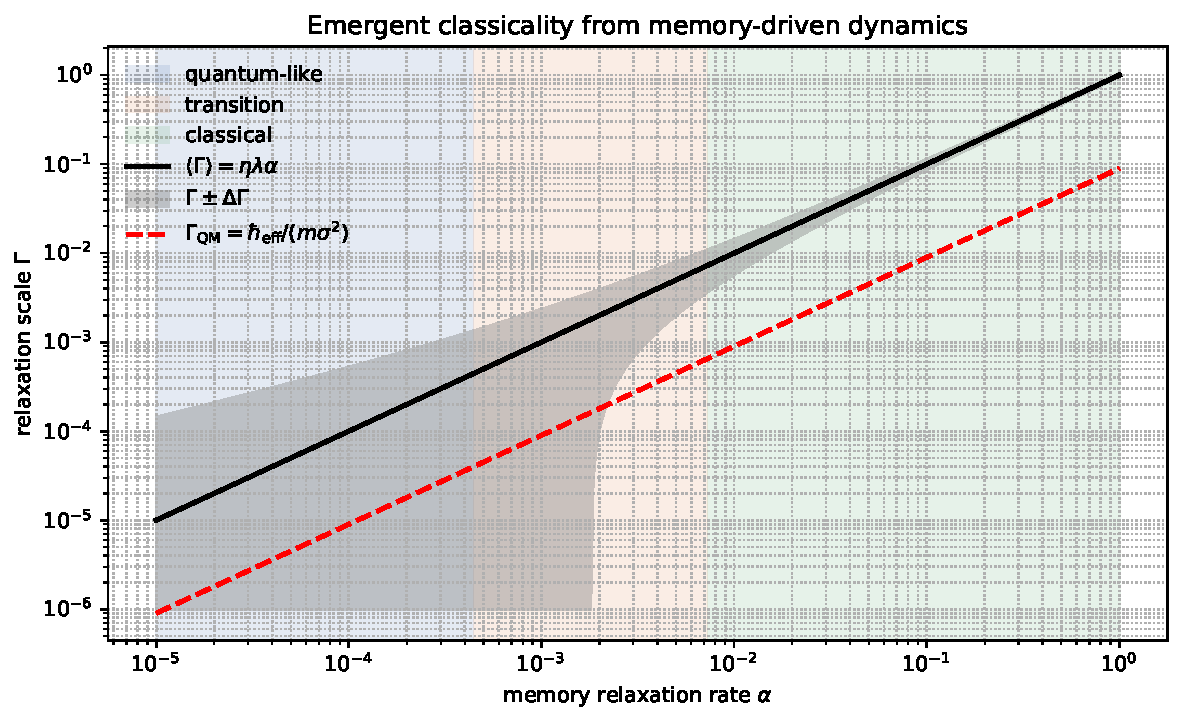
\includegraphics[width=0.9\linewidth]{../figures/paper/fig_Gamma_alpha.pdf}
    \caption{
    Crossover criterion between fluctuation-dominated and drift-dominated dynamics.
    The typical knot relaxation rate $\Gamma_{\mathrm{rel}}(\alpha)$ (set by memory-induced drift) competes with a stochastic uncertainty $\Delta\Gamma(\alpha)$ induced by fluctuations.
    Their ratio $R(\alpha):=\Gamma_{\mathrm{rel}}/\Delta\Gamma$ provides a natural control parameter distinguishing fluctuation-dominated ($R\ll 1$), crossover ($R\sim 1$), and drift-dominated ($R\gg 1$) regimes.
    }
    \label{fig:Gamma_alpha}
\end{figure}
Figures~\ref{fig:Gamma_alpha} and~\ref{fig:3d_knot_trajectory} summarize these regimes schematically and illustrate them with representative trajectories.
In Fig.~\ref{fig:Gamma_alpha}, $\Gamma_{\mathrm{rel}}$ denotes a typical knot relaxation rate induced by memory drift (operationally extractable, for instance, from an exponential fit to an in-knot autocorrelation $C(t)\propto e^{-\Gamma_{\mathrm{rel}} t}$ in the effective coarse-grained description), and $\Delta\Gamma$ its fluctuation-induced uncertainty estimated across windows or realizations. Their ratio $R=\Gamma_{\mathrm{rel}}/\Delta\Gamma$ serves as a drift-to-fluctuation control parameter.


\begin{figure}[htbp]
    \centering
    
\includegraphics[width=0.9\linewidth]{../figures/paper/fig_alpha.pdf}
    \caption{
    Schematic diagnostic map in the $(\varepsilon,\alpha)$-plane used for orientation in Paper~I.
    The background shading visualizes a dimensionless separation proxy distinguishing fluctuation-dominated from drift-dominated behavior and should not be read as a fundamental phase classification.
    A systematic derivation and its interpretation in terms of emergent Lorentzian structure are deferred to Paper~II.
    }
    \label{fig:alpha_phase}
\end{figure}

These qualitative differences are illustrated in Fig.~\ref{fig:3d_knot_trajectory}, where variations in the spatial organization of the trajectory reflect different regimes of memory persistence.

\begin{figure}[htbp]
    \centering
    
\includegraphics[width=0.95\linewidth]{../figures/paper/fig3_knot_trajectory.pdf}
    \caption{
    Organization of a trajectory into multiple knot-like regions in state space.
    The continuous line shows the full trajectory, while discrete points indicate sampled positions
    contributing to the memory distribution.
    Color denotes the update index $n$.
    Shown is a representative run illustrating metastable clustering; the qualitative behavior is robust across a range of parameters.
    }
    \label{fig:3d_knot_trajectory}
\end{figure}

\FloatBarrier

\subsection{Emergent time (coarse-graining)}\label{sec:EmergenceTime}

Although the update index $n$ is not physical time, the non-invertible memory dynamics makes the ordering of updates physically relevant.
The memory update rule Eq.~(\ref{eq:memorydistribution}) introduces a natural persistence scale of order $\alpha^{-1}$ update steps, which sets the coarse-graining resolution.
In regimes where coarse observables vary slowly on this scale, we use the effective (dimensionless) parameter
\begin{equation}\label{eq:t_taup}
t := \alpha n.
\end{equation}
Here $t$ counts (approximately) how many persistence scales have elapsed along the update sequence.
Correspondingly, since $\Delta t = \alpha$ per update step, differences in Eq.~(\ref{eq:trajectory}) may be approximated as
\begin{equation}
\frac{x_{n+1} - x_n}{\alpha}
\;\longrightarrow\;
\frac{\mathrm{d}x}{\mathrm{d}t}.
\end{equation}

This provides a convenient parametrization of the large-scale behavior of the discrete dynamics; different choices of coarse-graining correspond to different effective time resolutions.

A conceptual caveat: the extended state $z_n=(x_n,\rho_n)$ is Markov by construction, but the marginal process $\{x_n\}$ is generally non-Markovian because it depends on memory.

We stress that $t$ is, at this stage, an auxiliary coarse-grained parameter and remains dimensionless unless an additional calibration is introduced.
Moreover, in a strict continuum limit the discrete noise $\varepsilon\,\xi_n$ must be rescaled to yield a finite diffusion coefficient; a standard choice is a joint limit $\alpha\to 0$ and $\varepsilon\to 0$ at fixed $\varepsilon^2/\alpha$ (equivalently, fixed $D\sim \varepsilon^2/(2\alpha)$).

\subsection{Operational emergence of time}

The definition $t=\alpha n$ can be read purely as a reparametrization.
What makes it physically non-trivial in the present framework is that $\alpha^{-1}$ is not an externally supplied clock: it is an \emph{internally available} scale defined by the irreversible memory update, and it is operationally estimable from data of a single run (e.g., by the exponential forgetting rate of contributions to $\rho_n$).
In this sense, the continuum parameter $t$ is tied to a dynamical coarse-graining defined within the model, rather than being an independent fundamental input.

\subsubsection{Operational diagnostics}

The present work uses a small set of intrinsically defined, data-driven quantities for cross-run comparison:

- $\alpha$ is estimated from the exponential decay of memory weights in the linear update, i.e. by fitting the age-dependent factor $(1-\alpha)^m\simeq e^{-\alpha m}$ or by fitting the decay of a memory-sensitive observable such as $\Phi[\rho_n](x_n)$.
- $D$ is the effective diffusion coefficient of the coarse-grained dynamics, with the standard scaling estimate $D\sim\varepsilon^2/(2\alpha)$ in the continuum limit.
- $\Gamma_{\mathrm{rel}}$ is the knot relaxation rate extracted from the decay of an in-knot autocorrelation $C(t)\propto e^{-\Gamma_{\mathrm{rel}} t}$ or from the dominant relaxation eigenvalue of a quasi-stationary local linearization.
- $\widehat{\Gamma} := (\sigma^2/D)\,\Gamma_{\mathrm{rel}}$ is a dimensionless stability measure that compensates for uniform coordinate rescalings of the effective state space.

These diagnostics are intended to be operational: they can be estimated from simulation trajectories without assuming an a priori physical time unit.

\paragraph{Estimating $\alpha$ (and thus $t$) from a single trajectory.}
Because the memory update is linear and relaxing, the contribution of an update at step $k$ to later memory states $\rho_n$ is exponentially suppressed for $n\!>\!k$.
For the canonical update rule
\begin{equation}\label{eq:rho_linear_solution}
\rho_{n}=(1-\alpha)^{n-k}\rho_{k}
+\alpha\sum_{j=k+1}^{n}(1-\alpha)^{n-j}\,G_\sigma(x-x_{j})
\end{equation}
the weight of an ``impulse'' at age $m:=n-j$ scales as $(1-\alpha)^m\simeq e^{-\alpha m}$ for $\alpha\ll 1$.
Operationally, one may therefore estimate $\alpha$ by fitting an exponential decay law in $n$ for any memory-sensitive observable (e.g., the autocorrelation of a local functional of $\rho_n$ or of the induced drift $-\nabla\Phi[\rho_n](x_n)$), and then set $t:=\widehat{\alpha}\,n$ for cross-run comparisons.

Comparability between independent realizations can then be achieved by matching such intrinsic, dimensionless decay laws, which fixes the unit of $t$ up to statistical uncertainty.

Formally, one may write the coarse-grained dynamics as a stochastic differential equation
\begin{equation}
\mathrm{d}x = -\frac{\eta}{\alpha}\,\nabla\Phi[\rho(t)](x)\,\mathrm{d}t + \sqrt{2D}\,\mathrm{d}W_t,
\qquad
D \sim \frac{\varepsilon^2}{2\alpha},
\end{equation}
where $W_t$ is a standard Wiener process \cite{Oksendal2003,Risken1996}. We emphasize that the potential is induced by the memory field, $\Phi[\rho](x):=\int K(x,y)\rho(y)\,dy$, and is therefore slowly time-dependent in general.
In metastable knot regimes it may be treated as quasi-stationary on intermediate time scales. The precise numerical prefactor depends on conventions and on how the discrete-to-continuum limit is taken.

Unless stated otherwise, SDEs are interpreted in the It\^o sense.


\paragraph{Temporal direction and limits}
Because the memory update is irreversible, the coarse-grained parameter $t$ inherits a preferred direction: reversing $t$ does not correspond to a valid evolution of the discrete process.
Moreover, $t$ is useful only when memory relaxation provides a separation of scales.
For $\alpha\to 1$ memory becomes too short-lived for a controlled continuum description, while for $\alpha\to 0$ memory persists over arbitrarily long sequences and the coarse-graining becomes ambiguous.

In the regimes where a continuum description is meaningful, the next question is whether the dynamics self-organizes into robust metastable regions $\mathcal{K}\subset\Omega$.
We will quantify such ``dynamical knots'' operationally via the memory/visitation measure $M_n(\mathcal{K})$ and characterize their stability by an associated relaxation rate $\Gamma_{\mathrm{rel}}$.

%-------------------------------------------------
\section{Emergence of Mass and Dynamical Knots}
%-------------------------------------------------

Having established an effective notion of time, we now turn to the emergence of localized structures in the dynamics.
We show that stable, long-lived regions of the state space arise naturally as a result of memory-induced self-interaction, and that these structures motivate an operational ``mass'' proxy in terms of relaxation and stability diagnostics.

\subsection{Dynamical knots}

As illustrated in Figs.~\ref{fig:3d_knot_scatter} and~\ref{fig:3d_knot_trajectory}, the
trajectory generated by the update rules may organize into localized regions of repeated
visitation.
These regions are not imposed externally, but arise dynamically through the interplay of
stochastic motion and memory-induced drift.

\begin{figure}[htbp]
    \centering
    
\includegraphics[width=0.95\linewidth]{../figures/paper/fig2_knot_scatter.pdf}
    \caption{
    Scatter representation of sampled trajectory points illustrating clustering into knot-like regions in state space.
    Points show positions contributing to the memory distribution (coarse-grained at width $\sigma$).
    Color denotes the update index $n$.
    }
    \label{fig:3d_knot_scatter}
\end{figure}

We refer to such regions as \emph{dynamical knots}.
A dynamical knot is characterized by an enhanced local memory density Eq.~(\ref{eq:memorydistribution}) and a corresponding
self-consistent modification of the trajectory dynamics.
Importantly, a knot is not an object or a fixed point, but a stable dynamical pattern.
Operationally, a knot may be identified by a metastable region $\mathcal{K}\subset\Omega$ in which the coarse-grained visitation measure (equivalently, the memory density)
\begin{equation}
M_n(\mathcal{K}) := \int_{\mathcal{K}}\rho_n(x)\,dx
\end{equation}
remains elevated over many persistence times, e.g. $M_n(\mathcal{K})$ staying above a chosen threshold for $n$-intervals $\Delta n \gg \alpha^{-1}$.

Here $M_n$ is a region-level observable, while the induced potential $\Phi_n(x)=\int K(x,y)\rho_n(y)\,dy$ is a field on $\Omega$.
Intuitively, elevated $M_n(\mathcal{K})$ means that $\rho_n$ carries substantial mass near $\mathcal{K}$; through the convolution with $K$, this typically generates a locally restoring drift $-\nabla\Phi_n$ that stabilizes the knot.

In such regimes, the coarse-grained dynamics typically exhibits two distinct time scales: the memory persistence scale of order $\alpha^{-1}$ and a (potentially larger) knot relaxation scale $\tau_{\mathrm{rel}}$ characterizing return to the metastable region after perturbations.
Operationally, $\tau_{\mathrm{rel}}$ is defined with respect to the coarse-grained parameter $t$ (Sec.~\ref{sec:EmergenceTime}), e.g., by an exponential decay law of an in-knot autocorrelation $C(t)\propto e^{-t/\tau_{\mathrm{rel}}}$.
This motivates the later use of the relaxation rate $\Gamma_{\mathrm{rel}}:=1/\tau_{\mathrm{rel}}$ (and its dimensionless variant $\widehat{\Gamma}$) as an operational descriptor of knot stability.

\subsection{Attractors of the effective dynamics}

In the continuum description, the influence of memory may be summarized by an effective
potential $\Phi[\rho](x)$ induced by the memory field.
Dynamical knots correspond to regions where the gradient of this potential vanishes,
\begin{equation}
\nabla \Phi[\rho](x_\star) = 0,
\end{equation}
and small perturbations are suppressed. In the presence of stochastic forcing, knots are typically metastable (noise-broadened) attractor regimes rather than strictly stable fixed points.

The Hessian of the memory potential defined in Eq.~(\ref{eq:memorypotential}) determines the local relaxation rates. 
Linearizing the dynamics Eq.~(\ref{eq:trajectory}) around such a point $x_\star$ yields an OU-type approximation,
\begin{equation}
\mathrm{d}x = -\gamma H (x - x_\star)\,\mathrm{d}t + \sqrt{2D}\,\mathrm{d}W_t,
\end{equation}
where $H$ denotes the Hessian of the memory potential evaluated at $x_\star$, and
\begin{equation}
\gamma := \frac{\eta}{\alpha}
\end{equation}
collects the effective coupling to the memory-induced drift in the continuum description.

\paragraph{Remark (stability condition and time dependence).}
Strictly, $x_\star$ is a fixed point only for a \\emph{frozen} memory field (i.e., if $\rho$ is quasi-stationary on the relaxation time scale).
Local stability in the linearized (OU) approximation requires the symmetric part of $H$ to be positive definite (so that the drift is restoring) in the directions of interest; otherwise $x_\star$ is unstable or saddle-like and does not define a metastable knot.

This form describes a relaxation process toward the attractor, with characteristic decay
rates determined by the eigenvalues of $H$ \cite{Strogatz2018}.

\subsection{Effective mass as relaxation scale}

The stability of a dynamical knot is governed by the rate at which perturbations decay.
We therefore identify the effective mass associated with a knot not with resistance to acceleration, but with a relaxation scale characterizing the response of the system to fluctuations.

Concretely, in the coarse-grained (Markovian) regime one may define a characteristic relaxation time $\tau_{\mathrm{rel}}$ from linear response, e.g., from the decay of the autocorrelation of $x(t)$ within a metastable region.
Equivalently, $\tau_{\mathrm{rel}}$ can be obtained from the spectral gap of the linearized Fokker--Planck generator around the knot.
It is then natural to work with the associated relaxation rate
\begin{equation}
\Gamma_{\mathrm{rel}} := \frac{1}{\tau_{\mathrm{rel}}},
\end{equation}
with ``heavier'' knots corresponding to larger $\Gamma_{\mathrm{rel}}$ (faster relaxation, stronger confinement against fluctuations).

As a simple consistency check (and to remove coordinate-scaling ambiguities), one may report a dimensionless version using the intrinsic coarse-graining scales $\sigma$ and $D$ of the continuum description,
\begin{equation}
\widehat{\Gamma} := \frac{\sigma^2}{D}\,\Gamma_{\mathrm{rel}}.
\end{equation}
In knot regimes where a quasi-stationary linearization is valid, one expects $\Gamma_{\mathrm{rel}}$ to track the Hessian eigenvalue scale (Sec.~\emph{Mass as an attractor property} below), up to convention-dependent numerical factors.\looseness=-1
Moreover, under a uniform rescaling of coordinates $x\mapsto a x$ (with corresponding rescalings of the coarse-graining width $\sigma$), the dimensionless quantity $\widehat{\Gamma}$ should remain approximately invariant.
A sharper identification with a physical mass scale requires (and is deferred to later work) an emergent geometric calibration and an operational mapping to energy units.
\\paragraph{Terminology (``mass'' as an operational proxy).} We stress that ``mass'' here is not meant as a postulated inertial parameter of a background spacetime. Rather, it is a coarse-grained, quasi-time-independent property of a metastable attractor regime, quantified by how rapidly perturbations relax back into the knot. The terminology is therefore intentionally closer to ``stiffness'' or ``confinement strength'' than to Newtonian inertia; a mapping to conventional energy/mass units requires an additional calibration and is deferred to companion work.

\subsection{Metastability and transitions}

Not all knots are permanently stable.
Depending on the memory rate $\alpha$ and the strength of stochastic fluctuations, knots
may be metastable and decay over long but finite times \cite{Kramers1940,FreidlinWentzell2012}.
Transitions between different knot configurations correspond to qualitative changes in
the organization of the trajectory.

Such transitions are evident in Fig.~\ref{fig:3d_knot_trajectory}, where the trajectory
moves between distinct regions of enhanced memory feedback.
These processes will be shown to play a central role in the emergence of interaction
processes and effective dynamics at larger scales.

\subsection{Dimensionless diagnostics and effective scales}

The minimal dynamical model introduced in Sec.~\ref{sec:MinDynModel} is defined in terms of three parameters, $\varepsilon$, $\eta$, and $\alpha$, which characterize stochastic fluctuations, memory-induced drift, and memory relaxation, respectively.
We now summarize the effective scales and, crucially, dimensionless combinations that serve as operational diagnostics within the coarse-grained description.
A calibration of these scales to familiar physical constants and units is deferred to companion work.

\subsection{Diffusion and relaxation scales}

In the coarse-grained description, the stochastic contribution is summarized by an effective diffusion constant
\begin{equation}
D \sim \frac{\varepsilon^2}{2\alpha},
\end{equation}
(up to convention-dependent numerical factors). Together with the knot relaxation rate $\Gamma_{\mathrm{rel}}$ introduced above, the pair $(D,\Gamma_{\mathrm{rel}})$ forms a minimal set of effective scales that organize the metastable regimes discussed in this paper.

As an operational stability diagnostic we use the already defined dimensionless quantity $\widehat{\Gamma} := (\sigma^2/D)\,\Gamma_{\mathrm{rel}}$, which is approximately invariant under uniform coordinate rescalings $x\mapsto a x$ (with corresponding rescaling of $\sigma$).

The control ratio $R(\alpha)$ introduced in Fig.~\ref{fig:Gamma_alpha} may then be interpreted in terms of these effective scales as a drift-to-fluctuation diagnostic comparing $\Gamma_{\mathrm{rel}}$ to its fluctuation-induced uncertainty.

\subsection{Mass as an attractor property}

As discussed above, dynamical knots correspond to metastable (noise-broadened) attractor regimes of the effective dynamics.
Linearization around such an attractor point $x_\star$ yields, in the coarse-grained description, an OU-type stochastic relaxation law,
\begin{equation}
\mathrm{d}x = - \frac{\eta}{\alpha}\, H (x - x_\star)\,\mathrm{d}t + \sqrt{2D}\,\mathrm{d}W_t,
\end{equation}
where $H$ denotes the Hessian of the memory potential.

The characteristic relaxation rates are determined by the eigenvalues of the operator
$(\eta/\alpha)\, H$. Writing $\lambda$ for a characteristic eigenvalue of $H$, one has a typical relaxation rate
\begin{equation}
\Gamma_{\mathrm{rel}} \sim \frac{\eta}{\alpha}\,\lambda.
\end{equation}
This provides the link between the knot relaxation rate used in Fig.~\ref{fig:Gamma_alpha} and the Hessian eigenvalue scale of the linearized dynamics.

Since no metric is assumed on $\Omega$, the numerical value of $\lambda$ depends on the coordinate scaling of the state space. In practice, the kernel width $\sigma$ provides a natural reference scale, allowing one to form a dimensionless curvature measure $\tilde{\lambda} := \sigma^2\lambda$.

To connect relaxation to an energy-like scale without introducing additional postulates in the present paper, one may simply form the product
\begin{equation}
E_{\mathrm{rel}} \;:=\; 2D\,\Gamma_{\mathrm{rel}},
\end{equation}
which is controlled by the same two coarse-grained quantities that already appear in the OU approximation and in the dimensionless stability measure $\widehat{\Gamma}$. A calibration of $E_{\mathrm{rel}}$ to physical energy units (and its interpretation in terms of $mc^2$) is deferred to companion work.

In this formulation, mass is not a fundamental parameter but a measure of the stability of an attractor against stochastic perturbations.
Heavier structures correspond to steeper memory-induced potentials and/or stronger memory coupling, and thus faster relaxation.

%-------------------------------------------------
\section{Discussion and Outlook}
%-------------------------------------------------

We introduced a minimal self-interacting stochastic dynamics with finite, relaxing memory.
The non-invertibility of the memory update induces an intrinsic arrow of \emph{update order} without assuming thermodynamic irreversibility, physical time, or spacetime structure.
Coarse-graining on the memory-persistence scale yields an effective integration parameter $t=\alpha n$ and, when a separation of scales is present, a useful continuum SDE/FP approximation.

Within this effective regime, the dynamics generically self-organizes into localized, long-lived metastable structures (``dynamical knots'').
Their stability can be quantified operationally via relaxation rates, dimensionless stability measures, and residence-time statistics extracted directly from trajectories.
Interpreting such stability scales as mass-like proxies is natural at the level of the effective description, while any identification with physical units and relativistic structure is deferred to companion work.

Several limitations and open directions remain.
The continuum description is used here as an effective approximation rather than as a proven scaling limit; a rigorous convergence analysis, including conditions on $(G_\sigma,K)$ and parameter scalings, is left for future work.
A small NumPy reference implementation in `src/emergenz_knoten`, tests under `tests/`, and the reproducible runner `experiments/current/reference/reference_experiment.py` provide a concrete basis for verifying the numerical diagnostics reported in this draft.
Finally, extending the framework to multiple coupled generators and exploring when consistent universal scales emerge are natural next steps.

\begin{acknowledgments}
The author thanks colleagues for valuable feedback and discussion.
\end{acknowledgments}

% Use a BibTeX style that avoids RevTeX's journal abbreviation list warnings (jnrlst)
\bibliographystyle{unsrtnat}
\bibliography{references}

\end{document}
